\documentclass[../main.tex]{subfiles}




\begin{document}



\chapter{Bases de topologies}
\section{Bases}
\subsection{Bases. Definició i exemples}
\begin{defi}
[Base]\label{def:base}\index{Base} Sigui $\tau$ una topologia en un conjunt $X$. Una \textit{base} de $\tau$ (o de l'espai topològic $(X,\tau)$) és un subconjunt $\beta\subseteq \tau$ tal que tot element de $\tau$ és unió d'elements de $\beta$. És a dir,
\begin{equation}
    \notag
    \forall U\in \tau\;\exists\{U_i\}_{i\in I} \quad on\quad U_i\in \beta\;\forall i\in I\quad tq.\quad U = \bigcup_{i\in I}U_i.
\end{equation}
\end{defi}

A vegades direm \textit{elements bàsics}\index{Element bàsic} per a referir-nos a elements de la base.


Observem que, en general, $\tau$ conté molts més elements que $\beta$. No tot obert és necessàriament una bola oberta en aquest exemple. Observem també que un subconjunt de $\tau$ donat és base si, per començar és subconjunt (és a dir, que tot element de $\beta$ és de $\tau$) i si es compleix que tot element de $\tau$ és unió d'elements de $\beta$.

\begin{ej}
\label{ej:base1} Sigui $X$ un conjunt qualsevol no buit amb la topologia discreta $\tau = \mathscr{P}(X)$. Considerem la col·lecció
\begin{equation}
    \notag
    \beta = \{\{x\}\;:\;x\in X\} .
\end{equation}
Aleshores $\beta$ és una base de la topologia discreta. Vegem-ho: Primer, com que $\tau$ és la topologia discreta, tenim que tot subconjunt de $X$ és a $\tau$. Per tot $B = \{x\}\in\beta$, tenim aleshores,
\begin{equation}
    \notag
    B = \{x\}\in\beta\subseteq\tau. 
\end{equation}
Per a la segona condició, sigui $U\in\tau$. Aleshores, com $\tau$ és la topologia discreta, tenim que $U\subseteq X$. Per tot $x\in U$, tenim que $U$ pot ser expressat com la unió d'elements (que són conjunts) de $\beta$. En particular, per tot $U\in\tau$, tenim
\begin{equation}
    \notag
    U = \bigcup_{x\in U}\{x\}
\end{equation}
Així doncs, $\beta$ és una base de la topologia discreta.
\end{ej}

\begin{ej}
\label{ej:base2} Considerem el conjunt $X = \{a,b,c,d\}$ i la topologia 
\begin{equation}
    \notag
    \tau = \{\emptyset,\{a\},\{d\},\{a,d\},\{b,c\},\{a,b,c\},\{b,c,d\},X\}
\end{equation}
a $X$. Considerem la següent col·lecció d'oberts:
\begin{equation}
    \notag
    \beta = \{\{a\},\{d\},\{b,c\}\}
\end{equation}
Afirmem que $\beta$ és una base de $\tau$. En efecte, d'una banda és clar que tots els elements de $\beta$ són de $\tau$, és a dir, tots els elements de $\beta$ són oberts. D'altra banda, per veure la segona condició, només cal veure que els elements restants de $\tau$ que no són a $\beta$ poden ser expressats com a unió d'elements de $\beta$. Per conveni $\emptyset\in\beta$, o bé podem posar $\emptyset$ com la unió buida d'elements de $\beta$ i aleshores, en qualsevol cas, $\emptyset\in\tau$. Pels altres:
\begin{equation}
    \notag
    \{a\}\cup\{d\} = \{a,d\},\qquad \{a\}\cup\{b,c\} = \{a,b,c\},\qquad \{a\}\cup\{b,c\}\cup\{d\} = X.
\end{equation}
Així doncs, cada obert de $\tau$ és unió d'oberts de $\beta$ i així demostrem que $\beta$ és una base.
\end{ej}

\begin{ej}
\label{ej:base3} Sigui $\mathbb{R}$ amb $\tau_e$, la topologia euclidiana o usual dels intervals oberts de $\mathbb{R}$. Aleshores $\beta = \{(a,b)\;:\;a,b\in\mathbb{R},\;a<b\}$ és una base de $\tau_e$.

En efecte, notem que els oberts de $\mathbb{R}$ respecte $\tau_e$ són el conjunt buit $\emptyset$, el total $\mathbb{R}$, intervals oberts, unions arbitràries d'intervals oberts i interseccions finites d'intervals oberts. Ara hem de mirar que cadascun d'aquests oberts pot ser expressat com la unió d'elements de $\beta$. 

Aleshores, per conveni suposem que $\emptyset\in\beta$ o sinó podem interpretar $\emptyset$ com la unió buida d'elements de $\beta$. Ara, el total $\mathbb{R}$ pot ser obtingut com
\begin{equation}
    \notag
    \mathbb{R} = \bigcup_{\substack{a,b\in\mathbb{R}\\a<b}} (a,b).
\end{equation}
A més, cada interval $(a,b)\in\tau_e$ està contingut en $\beta$ perquè és la ``unió amb sí mateix''. Finalment considerem la unió d'un nombre arbitrari d'intervals $\{U_i\}_{i\in I}$ on $U_i = (a,b)$, per certs $a,b\in\mathbb{R}$, $a<b$, per a cada $i\in I$. Aleshores, $\bigcup_{i\in I} U_i$és la unió d'elements de $\beta$. Finalment, considerem la intersecció finita d'intervals de $\mathbb{R}$ oberts. La intersecció, com és finita, és o bé un interval obert o bé $\emptyset$ i els dos casos hem vist que es poden expressar com a unió d'elements de $\beta$. Per tant $\beta$ és una base de $\tau_e$.
\end{ej}

\begin{ej}
\label{ej:base4} Sigui $X$ un espai mètric qualsevol. Aleshores $\beta = \{B(x,\varepsilon)\;:\;x\in X,\;\varepsilon>0\}$ (la col·lecció de boles obertes en relació a la mètrica definida a $X$) és una base per la topologia resultant de la distància (topologia usual o euclidiana) a $X$.
\end{ej}

\begin{ej}
\label{ej:base5} Considerem $X = \{a,b,c,d\}$ i
\begin{equation}
    \notag
    \beta = \{\{a\},\{c,d\},\{a,b,c\}\}
\end{equation}
dos conjunts. Volem determinar si existeix alguna topologia $\tau$ a $X$ tal que $\beta$ en sigui una base. Això s'anticipa a un teorema que veurem properament.

Notem que, de principi, ningú ens diu que $\beta$ sigui una base de $\tau$ ja que de moment ni tan sols sabem si $\tau$ existeix. Donem totes les possibles unions d'elements de $\beta$:
\begin{equation}
    \notag
    \left\{
    \bigcup_{B\in\beta^*}B\;:\;\beta^*\subseteq\beta
    \right\}
    = \{\emptyset,\{a\},\{c,d\},\{a,b,d\},\{a,c,d\},X\} .
\end{equation}
Si $\tau$ és una topologia que té com a base $\beta$ ha de ser aquesta mateixa. Veiem, però, que
\begin{equation}
    \notag
    \{c,d\}\cap\{a,b,c\} = \{c\}\not\in\tau
\end{equation}
així que $\tau$ no pot ser cap topologia, ergo no existeix cap topologia que tingui el conjunt $\beta$ com a base.
\end{ej}

\begin{ej}
\label{ej:base6} Considerem l'espai topològic $(\mathbb{R},\tau)$ on $\tau$ és la topologia usual d'intervals oberts de $\mathbb{R}$. Volem veure que $\beta = \{(p,q)\;:\;p,q\in\mathbb{Q},\;p<q\}$ és una base. És suficient provar que qualsevol interval obert $(a,b)\in\tau$ pot ser expressat com a unió d'elements bàsics (elements de la base) ja que tot obert de $\tau$ és unió d'intervals oberts. Aleshores, sigui $(a,b)\in\tau$.
\begin{itemize}
    \item Si $a,b\in\mathbb{Q}$, aleshores $(a,b)\in\beta$ i ja hem acabat.
    \item Si $a\in\mathbb{Q}$, però $b\not\in\mathbb{Q}$, aleshores,
    \begin{equation}
        \notag
        (a,b) = \bigcup_{\substack{a<q<b\\q\in\mathbb{Q}}} (a,q).
    \end{equation}
    i per tant és unió d'elements de $\beta$.
    
    Anàlogament, si $b\in\mathbb{Q}$, però $a\not\in\mathbb{Q}$, aleshores,
    \begin{equation}
        \notag
        (a,b) = \bigcup_{\substack{a<p<b\\p\in\mathbb{Q}}} (p,b)
    \end{equation}
    i per tant és unió d'elements de $\beta$.
    
    \item Considerem el cas en què $a,b\not\in\mathbb{Q}$. Aleshores,
    \begin{equation}
        \notag
        (a,b) = \bigcup_{\substack{a<p<q<b\\p,q\in\mathbb{Q}}} (p,q)
    \end{equation}
    i, de nou, és unió d'elements de $\beta$.
\end{itemize}
\end{ej}

\begin{ej}
\label{ej:base7} Considerem un altre cop l'espai topològic $(\mathbb{R},\tau)$ on $\tau$ és la topologia usual d'intervals oberts a $\mathbb{R}$. Volem veure que $\beta = \{(w,z)\;:\;w,z\in\mathbb{Z},\;w<z\}$ \underline{\underline{NO}} és una base de $\tau$. En efecte, si $\beta$ fos una base de $\tau$ aleshores $\forall U\in\tau$ hauríem de trobar una col·lecció $\beta^*\subseteq\beta$ d'elements de $\beta$ tal que $U = \bigcup_{B\in\beta^*}B$. 

Considerem l'interval obert $U = (0,1/2)$. Qualsevol conjunt de $\beta$ contenint $U$ ha de ser tal que $w\leq 0$ i $1/2\leq z$. L'enter més petit $z$ satisfent-ho és $z = 1$ i aleshores l'element més petit de $\beta$ contenint $U$ és l'interval $(0,1)$. Però no hi ha conjunts en $\beta$ que estiguin continguts en $(0,1/2)$ i per tant $\beta$ no és una base de $\tau$.
\end{ej}

\subsection{Condició suficient per ser una base}
Recordem de la definició de base (\ref{def:base}) que si $(X,\tau)$ és un espai topològic, una base $\beta$ de $\tau$ és una col·lecció de subconjunts que són a $\tau$ tal que tot obert $U\in\tau$ és la unió d'elements de $\beta$.



\begin{prop}
\label{prop:condiciosuficientperserunabase} Sigui $(X,\tau)$ un espai topològic i $\beta\subseteq\tau$. Aleshores, $\beta$ és una base de $\tau$ si, i només si,
\begin{enumerate}[(1)]
    \item $\emptyset\in\beta$,
    \item $\forall U\in \tau$, $\forall x\in U$, $\exists B\in\beta$ tal que $x\in B\subseteq U$.
\end{enumerate}
\end{prop}
\begin{proof}
\begin{enumerate}[($\Leftarrow$)]
    \item Suposem que $\beta\subseteq \tau$ satisfà (1) i (2). Sigui $U\in\tau$. Si $U = \emptyset$ aleshores $U\in\beta$ i ja hem acabat. Suposem $U\not=\emptyset$. Prenem, per a cada $x\in U$, $B_x\in\beta$ tal que $x\in B_x\subset U$. Aleshores
    \begin{equation}
        \notag
        U = \bigcup_{x\in U}B_x
    \end{equation}
\end{enumerate}
\begin{enumerate}[($\Rightarrow$)]
    \item Recíprocament, si $\beta$ és una base, aleshores $\emptyset\in \beta$. Si $U\in\tau$, existeix $\{B_i\}_{i\in I}$ elements de $\beta$ tals que $U = \bigcup_{i\in I} B_i$. Si $x\in U$, $\exists i\in I$ tal que $x\in B_i\subseteq U$.
\end{enumerate}
\end{proof}

\begin{ej}
\label{ej:condiciosuficientperserunabase} Sigui $(X,\tau)$ un espai topològic on
\begin{equation}
    \notag
    X = \{a,b,c,d\}\quad\text{i}\quad\tau = \{\emptyset,\{a\},\{a,b\},\{a,b,c\},X\} .
\end{equation}
Volem determinar si $\beta = \{\{a\},\{a,b,c\}\}$ és una base de $\tau$. Utilitzant aquesta proposició (\ref{prop:condiciosuficientperserunabase}), si $\beta$ és base de $\tau$, aleshores per tot $U\in\beta$ i per tot $x\in U$, existeix $B\in\beta$ tal que $x\in B\subseteq U$.

Considerem el conjunt $U = \{a,b\}\in\tau$. Per tot $x\in U$, existeix $B\in\beta$ tal que $x\in B\subseteq U$? Per a $a\in U$ tenim $B_a = \{a\}\in\beta$ que és tal que $a\in B_a\subseteq U$. Però per a $b\in U$, tenim $b\not\in\{a\}$ i $b\in\{a,b,c\}\not\subseteq U$. Aleshores $\beta$ no pot ser una base de $\tau$.
\end{ej}

\subsection{Generant topologies a partir d'una col·lecció de subconjunts}
Fins ara per parlar de bases suposàvem que teníem fixat un espai topològic. Ara canviem el punt de vista. Sigui ara $X$ un conjunt i $\beta\subseteq \mathscr{P}(X)$. Ens podem preguntar si hi ha alguna topologia a $X$ de la qual $\beta$ sigui base. Observem que si $\beta$ és base d'una topologia $\tau$, aleshores forçosament
\begin{equation}
    \notag
    \tau = \tau_\beta:=\{\text{subconjunts de $X$ que es poden posar com a unió d'elements de $\beta$}\}.
\end{equation}

\begin{prop}
\label{prop:bases2} Sigui $X$ un conjunt i $\beta\subseteq\mathscr{P}(X)$. Aleshores, $\beta$ és base d'una topologia de $X$ (que necessàriament serà $\tau_\beta$) si, i només si, se satisfà:
\begin{enumerate}[(i)]
    \item $\emptyset\in\beta$,
    \item $X = \bigcup_{B\in\beta} B$,
    \item $\forall B,B'\in\beta$, $B\cap B'\in \tau_\beta$, és a dir, $B\cap B'$ és unió d'elements de $\beta$.
\end{enumerate}
\end{prop}
\begin{proof}
Hem vist que si $\tau$ existeix, aleshores 
\begin{equation}
    \notag
    \tau = \tau_\beta = \{Y\subseteq X\;:\;Y\text{ és unió d'elements de $\beta$}\} = \left\{\bigcup_{i\in I} U_i\;:\;\{U_i\}_{i\in I}\text{ elements de $X$}\right\}.
\end{equation}
Per tant, el lema és equivalent a dir que $\tau_\beta$ és una topologia si, i només si, se satisfan (i), (ii) i (iii).
\begin{enumerate}[($\Rightarrow$)]
    \item Si $\tau_\beta$ és una topologia, $\emptyset\in \tau_\beta$ que implica (i); $X\in\tau_\beta$ que implica (ii); i com que $\beta\subseteq\tau_\beta$, del fet que la intersecció de dos elements qualssevol de $\tau_\beta$ pertanyi a $\tau_\beta$, es dedueix (iii).
\end{enumerate}
\begin{enumerate}[($\Leftarrow$)]
    \item Suposem cert (i), (ii) i (iii). Aleshores $\emptyset\in\tau_\beta$ i $X\in\tau_\beta$. De la definició de $\tau_\beta$ es dedueix immediatament que la unió d'elements de $\tau_\beta$ pertany a $\tau_\beta$. Per veure que les interseccions de col·leccions finites d'elements de $\tau_\beta$ pertany a $\tau_\beta$ és suficient veure que 
    \begin{equation}
        \notag
        U,V\in\tau_\beta\Rightarrow U\cap V\in\tau_\beta
    \end{equation}
    Com que $U,V\in\tau_\beta$ vol dir que existeixen col·leccions $\{U_i\}_{i\in I}$ i $\{V_j\}_{j\in J}$ d'elements de $\beta$ tals que
    \begin{equation}
        \notag
        U = \bigcup_{i\in I} U_i,\qquad V = \bigcup_{j\in J} V_j
    \end{equation}
    aleshores
    \begin{equation}
        \notag
        U\cap V = \left(\bigcup_{i\in I} U_i\right)\cap\left(V = \bigcup_{j\in J} V_j\right) = \bigcup_{\substack{i\in I\\j\in J}} U_i\cap V_j
    \end{equation}
    on $U_i\cap V_j$ pertany a $\tau_\beta$ per (iii). Així doncs, $U\cap V\in\tau_\beta$.
\end{enumerate}
\end{proof}

\subsection{Comparació de topologies a partir de les seves bases}
\begin{lema}
\label{lema:dosbases} Suposem que $X$ és un conjunt i $\tau_1,\tau_2\subseteq\mathscr{P}(X)$ són topologies en $X$. Si $\beta_1$ és base de $\tau_1$ i $\beta_2$ és base de $\tau_2$, aleshores $\tau_1\subset \tau_2\Leftrightarrow \forall U\in\beta_1,\;\forall x\in U,\;\exists V\in\beta_2$ tal que $x\in V\subseteq U$.
\end{lema}
\begin{proof}
\begin{enumerate}[($\Rightarrow$)]
    \item Sigui $U\in\beta_1$, sigui $x\in U$. Volem provar que existeix $V\in\beta_2$ tal que $x\in V\subseteq U$.
    
    Com que $U\in\beta_1\subseteq\tau_1$ i $\tau_1\subset \tau_1$, aleshores $U\in\tau_2$. Com $\beta_2$ és base de $\tau_2$, aleshores $U$ és unió d'elements de $\beta_2$, és a dir, $\exists \{V_i\}_{i\in I}$, $V_i\in \beta_2$ tal que $U=\bigcup_{i\in I} V_i$ i com $x\in U$, ha d'estar en algun d'aquests $V_i$, és a dir, existeix $i_0\in I$ de forma que $x\in V_{i_0}\subset U$ i això és el que volíem.
\end{enumerate}
\begin{enumerate}[($\Leftarrow$)]
    \item Sigui $U\in\tau_1$. Volem veure que $U\in \tau_2$. Com que $\beta_1$ és base de $\tau_1$, aleshores $U$ és unió d'elements de $\beta_1$, és a dir, $U=\bigcup_{i\in I}U_i$, on $U_i\in \beta_1,\;\forall i\in I$. 
    
    Hem de veure que per tot $i\in I$, $U_i\in \tau_2$ i amb això obtindrem que la unió dels $U_i$, que és $U$, està a $\tau_2$.
    
    Per hipòtesis, donat $x\in U_i$, existeix un $V_{i,x}\in \beta_2$ tal que $x\in V_{i,x}\subseteq U_i$ per hipòtesis. Això es compleix per a tot $x$. Aleshores, $U_i = \bigcup_{x\in U_i} V_{i,x}$ i com $V_{i,x}\in \beta_2$, la unió d'aquests elements és un element de $\tau_2\Rightarrow U_i\in \tau_2$. Això per a tota $i\in I$. Per tant, $U\in\tau_2$.
\end{enumerate}
\end{proof}

\begin{ej}
Sigui $(X,d)$ un espai mètric i sigui $\tau$ la topologia donada per $d$. Sigui $Y$ un subconjunt de $X$. Hi ha dues maneres de definir una topologia a $Y$:
\begin{enumerate}[(1)]
    \item $\tau_Y$, la topologia induïda per $Y$ (veure (\ref{def:topologiasubespai})).
    \item Sigui $d_Y = d_{|Y\times Y}$, aleshores $(Y,d_Y)$ és un espai mètric i podem prendre a $Y$ la topologia $\tau_Y'$ induïda per $d_Y$. Aleshores, $\tau_Y = \tau_Y'$.
    
    (En general, si $\beta$ és una base de $X$ i $Y\subseteq X$, el conjunt $\{B\cap Y\;:\;B\in \beta\}$ és una base de la topologia induïda a $Y$).
    \begin{proof}
    Prenem
    \begin{equation}
        \notag
        \begin{array}{ll}
            \beta_Y = \{B_r^d(x)\cap Y\;:\; r>0\;x\in X\}\quad \text{base de $\tau_Y$} \\
            \beta_Y' = \{B_\rho^{d_Y}(y)\;:\;\rho>0,\;y\in Y\}
        \end{array}
    \end{equation}
    Com que $d_Y = d_{|Y\times Y}$, $\beta_Y'\subseteq \beta_Y$. D'altra banda, si prenem $r>0$, $x\in X$, $y\in B_r^d(x)\cap Y$, aleshores prenem $\rho = r-d(y,x)>0$ se satisfà $y\in B_\rho^{d_Y}(y)\subseteq B_r^d(x)\cap Y$. Això demostra que $\tau_Y = \tau_Y'$.
    \end{proof}
\end{enumerate}
\end{ej}

\section{Subbases}

Recordem que una base d'un espai topològic $(X,\tau)$ és una col·lecció $\beta\subseteq\tau$ tal que $\forall U\in\tau$ es pot escriure com a unió d'elements de $\tau$, és a dir, $\forall U\in\tau$, $\exists\beta^*\subseteq\beta$ tq. $U = \bigcup_{B\in\beta^*}B$. Ara definirem un terme general anomenat subbase.

\begin{defi}[Subbase]
\label{def:subbase}\index{Subbase} Sigui $(X,\tau)$ un espai topològic. Una col·lecció $S\subseteq\tau$ es diu \textit{subbase} (en anglès: subbase o subbasis) de $\tau$ si el conjunt d'interseccions finites d'elements de S formen una base de $\tau$. És a dir, si 
\begin{equation}
    \notag
    \beta_S = \{U_1\cap U_2\cap\cdots\cap U_k\;:\;U_1,\ldots,U_k\in S\}
\end{equation}
és base de $\tau$.
\end{defi}

La següent proposició ens dona una definició alternativa.

\begin{prop}
\label{prop:subbase} Sigui $(X,\tau)$ un espai topològic. $S$ és una subbase de $\tau$ si, i només si, $\tau$ és la topologia més petita contenint $S$.
\end{prop}

\begin{ej}
\label{ej:subbase1} Considerem l'espai topològic $(\mathbb{R},\tau)$ on $\tau$ és la topologia d'intervals oberts a $\mathbb{R}$. Considerem el següent conjunt d'intervals semi-infinits:
\begin{equation}
    \notag
    S = \{(-\infty,b)\;:\;b\in\mathbb{R}\}\cup\{(a,+\infty)\;:\;a\in\mathbb{R}\}\cup\{\mathbb{R}\} .
\end{equation}
Notem que per $a,b\in\mathbb{R}$, $a<b$, tenim $(-\infty,b)\cap(a,+\infty) = (a,b)$. Per $a\geq b$ tenim $(-\infty,b)\cap(a,+\infty) = \emptyset$. Així doncs, la col·lecció de totes les interseccions finites d'elements de $S$ són o bé intervals oberts o bé $\emptyset$. Recordem que la col·lecció d'intervals oberts ja sabem que forma una base de $\tau$ (usual) en $\mathbb{R}$. Per tant, $S$ és una subbase de $\tau$ ja que $\beta_S$ és base de $\tau$.
\end{ej}

\begin{ej}
\label{ej:subbase2} Considerem el conjunt $X = \{a,b,c,d,e,f\}$ amb la topologia
\begin{equation}
    \notag
    \tau = \{\emptyset,\{a\},\{c,d\},\{a,c,d\},\{b,c,d,e,f\},X\} .
\end{equation}
Volem veure que el subconjunt $S = \{\{a\},\{a,c,d\},\{b,c,d,e,mf\}\}\subseteq \tau$ és una subbase de $\tau$.

La col·lecció de totes les possibles interseccions finites entre elements de $S$ és
\begin{equation}
    \notag
    \beta_S = \{\emptyset,\{a\},\{c,d\},\{a,c,d\},\{b,c,d,e,f\}\} .
\end{equation}
Tots els altres elements de $\tau$ són unions trivials d'elements de $\beta_S$ i $X = \{a\}\cup\{b,c,d,e,f\}$ així que $\beta_S$ és una base i per tant $S$ una subbase de $\tau$.
\end{ej}

\begin{ej}
\label{ej:subbase3} Sigui $X = \{a,b,c,d,e\}$ i $\tau = \{\emptyset,\{a\},\{b\},\{a,b\},\{a,b,d\},\{a,b,c,d\},X\}$. Volem veure que 
\begin{equation}
    \notag
    S = \{\{a\},\{b\},\{a,b\},\{a,b,d\},\{a,b,c,d\},X\}
\end{equation}
\underline{\underline{NO}} és una subbase. Considerem $\beta_S$ el conjunt de totes les interseccions finites dels elements de $S$:
\begin{equation}
    \notag
    \beta_S = \{\emptyset,\{a\},\{b\},\{a,b\},\{a,b,d\},\{a,b,c,d\},X\} .
\end{equation}
Veiem que tots els conjunts que hi ha, excepte $\{b,d\}$, poden ser expressats com a unió d'elements de $\tau$. Però aquest $\{b,d\}$ no, i per tant $\beta_S$ no és base de $\tau$, ergo $S$ no és subbase de $\tau$.
\end{ej}

\section{Entorns i bases d'entorns}
\subsection{Entorn d'un punt en un espai topològic}

\begin{defi}
[Entorn]\label{def:entorn}\index{Entorn} Sigui $X$ un espai topològic i $x\in X$. Un \textit{entorn} de $x$ és un subconjunt $E\subseteq X$ tal que $x\in E^{o}$.
\end{defi}

En altres paraules, un entorn d'un punt $x\in X$, és un conjunt $E\subseteq X$ per al qual existeix un obert $U\subseteq E$ tal que $x\in U$. Es diu entorn obert d'un punt $x\in X$ a qualsevol conjunt obert $U\in\tau$ tal que $x\in U$.

Sovint, però, el terme ``entorn'' s'utilitza volent dir ``entorn obert'' quan la distinció no és important.

Amb aquesta definició podem obtenir el següent criteri per veure si un conjunt és obert:

\begin{prop}
\label{prop:entorn1} Sigui $(X,\tau)$ un espai topològic i sigui $U\subseteq X$. Aleshores $U$ és obert si, i només si, $\forall x\in U$, $\exists U_x$ entorn obert de $x$ tal que $U_x\subseteq U$.
\end{prop}
\begin{proof}
\begin{enumerate}[($\Rightarrow$)]
    \item Suposem que $U$ és obert. Aleshores, per tot $x\in U$, sigui $U_x = U$. Això ja compleix el que volíem: $U_x$ és un entorn de $x$ obert tal que $U_x\subseteq U$.
\end{enumerate}
\begin{enumerate}[($\Leftarrow$)]
    \item Suposem que per a tot $x\in U$ existeix un entorn obert $U_x$ de $x$ tal que $U_x\subseteq U$. Aleshores, $U = \bigcup_{x\in U}U_x$. Com la unió arbitrària d'oberts és un obert, tenim que $U$ és obert.
\end{enumerate}
\end{proof}

\begin{prop}
\label{prop:entorn2} Sigui $(X,\tau)$ un espai topològic i $C\subseteq X$. Aleshores $C$ és tancat si i només si per a tot $x\in X\setminus C$ existeix un entorn obert $U_x$ de $x$ tal que $U_x\subseteq X\setminus C$. Equivalentment, $C$ és tancat si i només si per tot $x\in X\setminus C$ existeix un entorn obert $U_x$ de $x$ tal que $U_x\cap C = \emptyset$.
\end{prop}
\begin{proof}
Com $C$ és tancat, $X\setminus C$ és obert, i el resultat se segueix de la proposició (\ref{prop:entorn1}).
\end{proof}

\begin{ej}
\label{ej:entorn1} Considerem el conjunt finit $X = \{a,b,c\}$ i la topologia $\tau = \{\emptyset,\{a\},\{a,b\},$ $X\}$. Considerem l'element $a\in X$. Els entorns oberts de $a$ són $\{a\}, \{a,b\}$ i $\{a,b,c\}=X$. Ara considerem l'element $b\in X$. Els entorns oberts de $b$ són $\{a,b\}$ i $\{a,b,c\}$. Finalment, l'únic entorn obert de $c$ és $X$.
\begin{equation}
    \notag
    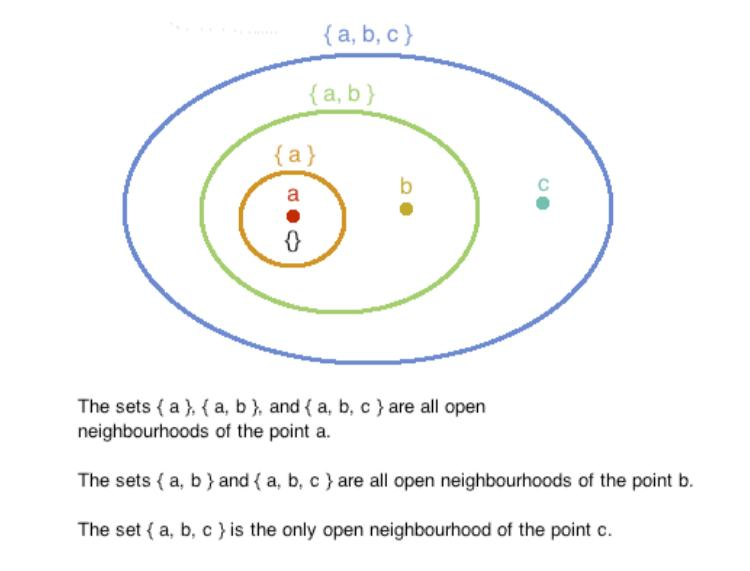
\includegraphics[scale = 0.2]{fotos_topo_1/entornexemple1.jpeg}
\end{equation}
\end{ej}

\begin{ej}
\label{ej:entorn2} Considerem $X=\mathbb{Z}$ amb la topologia dels complements finits:
\begin{equation}
    \notag
    \tau = \{\emptyset\}\cup\{U\subseteq\mathbb{Z}\;:\;\mathbb{Z}\setminus U\;\text{és finit}\}
\end{equation}
Considerem el punt $1\in\mathbb{Z}$. Sigui $A\subseteq \mathbb{Z}$ un conjunt finit. Aleshores qualsevol conjunt de la forma $\{1\}\cup (\mathbb{Z}\setminus A)$ és un entorn obert de $1$. Per veure això, notem que com $A$ és finit, $\mathbb{Z}\setminus A$ és un conjunt infinit sense els elements d'$A$. Així doncs, $\{1\}\cup (\mathbb{Z}\setminus A)$ és també un conjunt infinit que conté tots els elements excepte els d'$A$ i amb l'1 afegit de nou. El complementari d'aquest conjunt és
\begin{equation}
    \notag
    (\{1\}\cup(\mathbb{Z}\setminus A))^c = A\setminus\{1\}
\end{equation}
Com $A$ és finit, $A\setminus\{1\}$ també és finit i per tant $\{1\}\cup(\mathbb{Z}\setminus A)\in\tau$ és un obert. Més enllà, tenim que $1\in\{1\}\cup(\mathbb{Z}\setminus A)$. Així doncs, cada conjunt de la forma $\{1\}\cup(\mathbb{Z}\setminus A)$ on $A\subseteq\mathbb{Z}$ és finit, és un entorn obert de 1.
\end{ej}

\begin{ej}
\label{ej:entorn3} Considerem l'espai topològic $(\mathbb{R},\tau)$ on $\tau = \{(-n,n)\;:\;n\in\mathbb{N},\;n\geq 1\}$. Volem descriure tots els entorns oberts de $\pi\in\mathbb{R}$. La col·lecció de tots els oberts d'aquesta topologia és
\begin{equation}
    \notag
    \tau = \{(-1,1),(-2,2),\ldots,(-n,n),\cdots\}
\end{equation}
A més, veiem que els oberts estan ``encadenats'' de la següent manera
\begin{equation}
    \notag
    (-1,1)\subset(-2,2)\subset\cdots\subset(-n,n)\subset\cdots\subset\mathbb{R}
\end{equation}
Observem que $\pi\not\in(-1,1)$, $\pi\not\in(-2,2)$, $\pi\not\in(-3,3)$, però $\pi\in(-4,4)$. I aleshores, pel que hem vist de la cadena, $\pi\in(-n,n),\;\forall n\geq 4$. Per tant, una col·lecció d'entorns oberts de $\pi\in\mathbb{R}$ és $\{(-n,n)\;:\;n\geq 4\}$
\end{ej}

\begin{ej}
\label{ej:entorn4} Sigui $X$ un conjunt finit no buit de $n$ elements i considerem l'espai topològic $(X,\tau)$ on $\tau$ és la topologia discreta en $X$. Veiem que $x\in X$ té $2^{n-1}$ entorns oberts.

En efecte, si $\tau$ és la topologia discreta, aleshores $\tau = \mathscr{P}(X)$. Per tant $\#\tau = 2^n$. Sigui $x\in X$. Per tot $A\in\tau=\mathscr{P}(X)$ tenim que, o bé $x\in A$, o bé $x\not\in A$. Així doncs, $\mathscr{P}(X)$ es pot dividir en dos grups d'iguals dimensions: $2^n/2 = 2^{n-1}$. El primer grup de conjunts contenint $x$ i el segon grup de conjunts que no contenen $x$. Així doncs, hi ha $2^{n-1}$ subgrups de $X$ que contenen $x$, però cada conjunt de $X$ és un obert, per tant hi ha $2^{n-1}$ entorns oberts de $x$, per tot $x\in X$.
\end{ej}

\begin{ej}
\label{ej:entorn5} Considerem l'espai topològic $(\mathbb{Z},\tau)$ on $\tau$ és la topologia dels complements numerables. Quins són els entorns de $1\in\mathbb{Z}$? I quin n'és el més petit? El conjunt d'entorns oberts de 1 és una col·lecció de conjunts de $\tau$ contenint 1. Notem que $\mathbb{Z}$ és un conjunt numerable. Aleshores, per tot $A\subseteq\mathbb{Z}$ tenim que $A^c = \mathbb{Z}\setminus A$ es un conjunt numerable. Per tant, tot $A\subseteq \mathbb{Z}$ és un obert. Així doncs, tot subconjunt de $\mathbb{Z}$ contenint 1 és un entorn obert de 1. Per exemple, el conjunt dels enters imparells
\begin{equation}
    \notag
    (2n+1)\mathbb{Z} = \{\ldots,-3,-1,1,3,\ldots\}
\end{equation}
és un entorn obert de 1. El conjunt de quadrats $S =\{1,4,9,\ldots\}$ també n'és un entorn obert. Aleshores, és clar que l'entorn obert més petit de 1 és $\{1\}$.
\end{ej}

\begin{ej}
\label{ej:entorn6} Considerem l'espai topològic $(\mathbb{R},\tau)$ on $\tau$ és la topologia dels complements numerables. Veurem dos exemples d'entorns oberts de $1\in\mathbb{R}$. Els entorns oberts de 1 són els oberts contenint 1. Considerem el conjunt
\begin{equation}
    \notag
    A = (\mathbb{R}\setminus N)\cup\{1\} .
\end{equation}
Aleshores $A^c = \mathbb{N}\setminus\{1\}$ és numerable.

Per un altre exemple, considerem el conjunt $B = \mathbb{R}\setminus\{2\}$. Aleshores $B^c = \{2\}$ que és numerable així que $B\in\tau$ i $1\in B$, per tant $B$ és un entorn obert de 1.

De fet, per qualsevol $b\in\mathbb{R}$ on $b\not=1$, si definim $B_b = \mathbb{R}\setminus\{b\}$, aleshores $B_b^c = \{b\}$ que és numerable i per tant $B_b\in\tau$ i $1\in B_b$. Aleshores $B_b$ és un entorn obert de 1, ja que $1\in B_b$, $\forall b\in\mathbb{R}\setminus\{1\}$.
\end{ej}

\begin{ej}
\label{ej:entorn7} Considerem el conjunt $X = \{a,b,c,d,e\}$. Volem trobar una topologia no discreta $\tau$ a $X$ tal que $a,b\in X$ comparteixin exactament tres entorns oberts.

Si $a$ i $b$ comparteixen exactament 3 entorns oberts aleshores ha d'haver-hi 3 oberts contenint els dos elements, $a$ i $b$. Considerem la següent topologia:
\begin{equation}
    \notag
    \tau = \{\emptyset,\{d\},\{a,b,c\},\{a,b,c,d\},X\} .
\end{equation}
Aleshores,
\begin{equation}
    \notag
    a,b\in U_1 = \{a,b,c\},\qquad a,b\in U_2 = \{a,b,c,d\},\qquad a,b\in U_3 = \{a,b,c,d,e\}
\end{equation}
i per tant comparteixen exactament tres entorns oberts, com volíem. Caldria provar que $\tau$ és efectivament una topologia.
\end{ej}

\subsection{Bases d'entorns}

Recordem que si $(X,\tau)$ és un espai topològic, una base $\beta$ de $\tau$ és una subcol·lecció de $\tau$ tal que tot $U\in\tau$ és la unió d'alguna subcol·lecció $\beta^*\subseteq \beta$ de $\beta$, és a dir, $\forall U\in\tau$, $\exists \beta^*\subseteq\beta$ tal que $U = \bigcup_{B\in\beta^*}B$. Ara estudiarem una definició similar.

\begin{defi}
[Base d'entorns]\label{def:basedentorns}\index{Base d'entorns} Una \textit{base d'entorns} (o sistema fonamental d'entorns o base local) de $x$ és una col·lecció d'entorns (oberts) de $x$, $\{E_i\}_{i\in I}$, amb la propietat que per tot entorn $E$ de $x$ existeix $i\in I$ tal que $E_i\subseteq E$.
\end{defi}

En altres paraules, una base d'entorns del punt $x\in X$ és una col·lecció de conjunts $\beta_x$ tal que per tot entorn obert de $x$ existeix un element bàsic $B\in\beta_x$ contingut a aquest entorn obert.
\begin{equation}
    \notag
    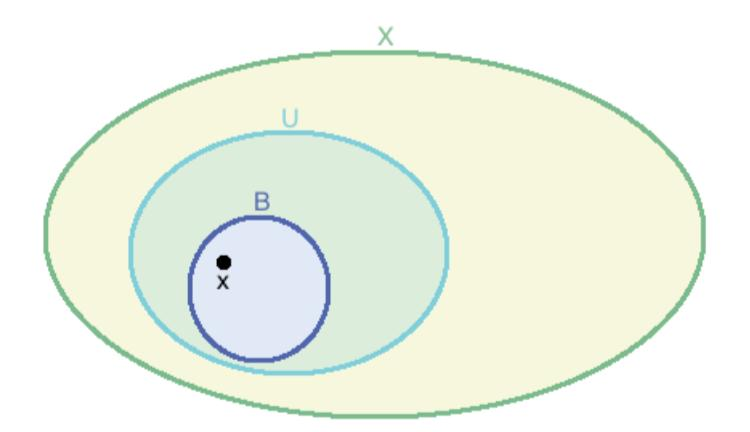
\includegraphics[scale = 0.3]{fotos_topo_1/baseentorn.jpeg}
\end{equation}


\begin{ej}
\label{ej:baseentorn1} Considerem l'espai topològic $(\mathbb{R},\tau)$ on $\tau$ és la topologia usual dels intervals oberts a $\mathbb{R}$. Considerem el punt $0\in\mathbb{R}$. Una base d'entorns de 0 és la col·lecció
\begin{equation}
    \notag
    \beta_0 = \{(a,b)\;:\;a<0<b\} .
\end{equation}
Per exemple, si considerem l'obert $U = (-1,1)\cup(2,3)\in\tau$ que conté el 0, aleshores per a $B = (-1/2,1/2)\in\beta_0$ tenim que $0\in B\subseteq U$.

Més en general, per a tot $x\in\mathbb{R}$, una base d'entorns de $x$ és
\begin{equation}
    \notag
    \beta_x = \{(a,b)\;:\;a<x<b\} .
\end{equation}
Això és perquè per qualsevol obert $U\in\tau$ contenint $x$, existirà un interval obert contenint $x$ que estigui contingut en $U$.
\end{ej}

\begin{ej}
\label{ej:baseentorn2} Considerem el conjunt $X =\{a,b,c,d,e\}$ i la topologia
\begin{equation}
    \notag
    \tau = \{\emptyset,\{a\},\{a,b\},\{a,c\},\{a,b,c\},\{a,b,c,d\},X\} .
\end{equation}
Què és una base d'entorns per a l'element $b\in X$? Primer mirem els conjunts de $\tau$ que continguin $b$. Aquests són
\begin{equation}
    \notag
    U_1 = \{a,b\},\qquad U_2 = \{a,b,c\},\qquad U_3 = \{a,b,c,d\},\qquad U_4 = X.
\end{equation}
Veiem que $\beta_b = \{\{b\}\}$ pot funcionar com a base d'entorns de $b$ ja que
\begin{equation}
    \notag
    b\in\{b\}\subseteq U_1,\quad b\in\{b\}\subseteq U_2,\quad b\in\{b\} \subseteq U_3,\quad b\in\{b\} \subset U_4= X.
\end{equation}
Quina seria una base de $c$? Els conjunts de $\tau$ contenint $C$ són $V_1 = \{a,c\}$, $V_2  = \{a,b,c\}$, $V_3 = \{a,b,c,d\}$ i $V_4 = X$. Veiem que $\beta_c = \{\{a,c\}\}$ funciona com a base d'entorns de $c$ ja que
\begin{equation}
    \notag
    c\in\{a,c\}\subset V_i,\quad i=1,2,3,4.
\end{equation}
\end{ej}

\begin{prop}
\label{prop:baseentorn1} Sigui $(X,\tau)$ un espai topològic i sigui $\beta$ una base de $\tau$. Aleshores, per tot $x\in X$, $\beta_x = \{B\in\beta\;:\;x\in B\}$ és una base d'entorns de $x$.
\end{prop}
\begin{proof}
Sigui $x\in X$ i sigui $\beta_x = \{B\in\beta\;:\;x\in B\}$. Per veure que $\beta_x$ és una base d'entorns de $x$ hem de veure que per tot $U\in\tau$ amb $x\in U$ existeix $B\in\beta_x$ tal que $x\in B\subseteq U$.

Sigui $U\in\tau$ amb $x\in U$. Com $\beta$ és una base de $\tau$, tenim que existeix una subcol·lecció $\beta^*\subseteq \beta$ tal que $U = \bigcup_{B\in\beta^*}B$. Com $x\in U$, tenim que $x\in\bigcup_{B\in\beta^*}B$. Per tant, $x$ està a al menys un dels $B\in\beta^*$. Sigui $B_x$ aquest tal que $x\in B_x\in\beta^*$. Aleshores, $B_x\in\beta_x$ ja que $x\in B_x$ i $B_x\in\beta^*\subseteq\beta$ i per tant
\begin{equation}
    \notag
    x\in B_x\in\bigcup_{B\in\beta^*}B = U.
\end{equation}
Així doncs, per tot $U\in\tau$ amb $x\in U$, existeix $B_x\in\beta_x = \{B\in\beta\;:\;x\in B\}$ tal que $x\in B_x\subseteq U$. Aleshores $\beta_x$ és una base d'entorns de $x$.
\end{proof}

\begin{prop}
\label{prop:baseentorn2} Sigui $(X,\tau)$ un espai topològic. Si $\{\beta_x\}_{x\in X}$ és una col·lecció de bases d'entorns per cada $x\in X$, aleshores 
\begin{equation}
    \notag
    \beta = \bigcup_{x\in X}\beta_x
\end{equation}
és una base de $\tau$.
\end{prop}
\begin{equation}
    \notag
    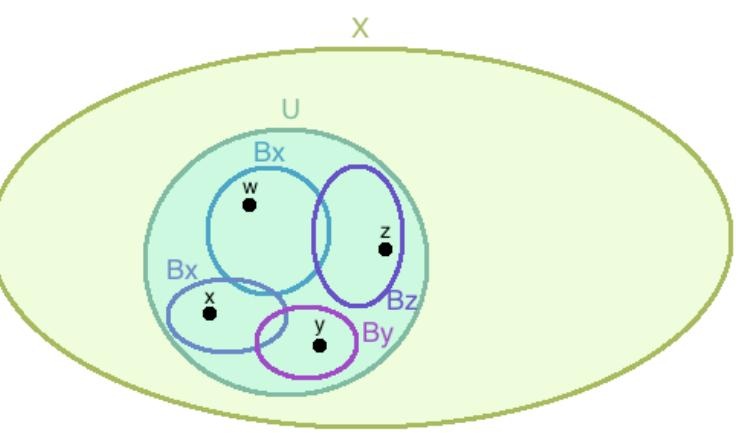
\includegraphics[scale = 0.3]{fotos_topo_1/baseentorn2.jpeg}
\end{equation}
Per cada obert $U$ i per a tot element $x$ de $U$ considerem la base d'entorns de $x$, $\beta_x$. Com $\beta_x$ és base d'entorns de $x$, tenim un conjunt $B_x$ de $\beta_x$ tal que $x\in B_x$ i $B_x\subseteq U$. La unió de tots aquests $B_x$ en $\beta_x$ $\forall x\in U$ ens mostra que $U$ pot ser escrit com la unió d'elements de $\beta$ (la unió de tots els $\beta_x$ per tot $x\in U$).
\begin{proof}
Sigui 
\begin{equation}
    \notag
    \beta = \bigcup_{B\in\beta}B.
\end{equation}
Recordem que $\beta$ és una base de la topologia $\tau$ si per tot $U\in\tau$, existeix una subcol·lecció de $\beta$ tal que $U$ n'és la unió dels seus elements.

Sigui $U\in\tau$ i $x\in  U$. Aleshores existeix una base d'entorns de $x$, $\beta_x\subseteq \beta$. Com $\beta_x$ és una base d'entorns de $x$, tenim que per $U\in \tau$ existeix un $B_x\in\beta_x$ tal que $x\in B_x\subseteq U$. Així que tenim:
\begin{equation}
    \notag
    U = \bigcup_{x\in U}B_x
\end{equation}
Per tant, tot $U\in\tau$ pot ser expressat com la unió d'elements de $\beta$, així $\beta = \bigcup_{x\in X}\beta_x$ és una base de $\tau$.
\end{proof}

\section{Axiomes de numerabilitat}
\subsection{Recordatori dels conjunts numerables}
Recordem:
\begin{defi}
[Conjunt numerable]\label{def:numerable}\index{Conjunt numerable} Direm que un conjunt $X$ és numerable si existeix una aplicació bijectiva $X\rightarrow \mathbb{N}$ (és a dir, una bijecció entre $X$ i el conjunt dels naturals, de forma que se li pot assignar a cada element de $X$ un cardinal).
\end{defi}

\begin{nota}
\label{nota:numerable} Observem
\begin{itemize}
    \item Numerable no vol dir finit. Per exemple: $\mathbb{N}, \mathbb{Q}, \mathbb{Z}$ són numerables i infinits.
    \item Els conjunts finits no tenen per què ser numerables. Per exemple, els intervals de $\mathbb{R}$ són finits i no numerables, per petits que siguin.
\end{itemize}
\end{nota}

\begin{prop}
\label{prop:propietatsnumerable} Propietats:
\begin{itemize}
    \item Si $X,Y$ són numerables, aleshores $X\times Y$ són numerables. Més general, per a $n\in\mathbb{N}$, si $A_1,\ldots,A_n$ són numerables, aleshores $A_1\times \cdots\times A_n$ és numerable.
    \item Si $X$ és numerable i $Y\subseteq X$ és un subconjunt, aleshores $Y$ és numerable. Si $Y$ no és numerable i $Y\subseteq X$, aleshores $X$ no és numerable.
    \item Si $I$ és numerable i $\{A_i\}_{i\in I}$, $A_i$ numerable, aleshores $\bigcup_{i\in I}A_i$ és numerable.
\end{itemize}
\end{prop}

Ara enunciem els axiomes.

\subsection{Primer axioma de numerabilitat}
\begin{defi}
[Primer axioma de numerabilitat (1AN)]\label{def:1an}\index{Primer axioma de numerabilitat (1AN)} Sigui $(X,\tau)$ un espai topològic. Direm que verifica el \textit{primer axioma de numerabilitat} si  per a cada $p\in X$, existeix $\beta_p$ una base d'entorns de $p$ numerable.
\end{defi}

\begin{ej}
\label{ej:1an1} Considerem l'espai topològic $(\mathbb{R},\tau)$, on $\tau$ és la topologia usual dels intervals oberts en $\mathbb{R}$. Afirmem que aquest espai topològic satisfà el 1AN.

Per veure-ho, sigui $x\in X$. Aleshores, tot obert que contingui $x$ ha de contenir un interval obert $(a,b)$ de $\mathbb{R}$ contenint $x$, és a dir, tal que $x\in (a,b)$. Definim la base d'entorns per $x$ com
\begin{equation}
    \notag
    \beta_x = \{B_{x_n} = (x-1/n, x+1/n)\;:\;n\in\mathbb{N}\}
\end{equation}
Per tant, per cada $U\in\tau$ tal que $x\in U$ tenim $x\in (a,b)\subseteq U$ i, de fet, existeix $n\in\mathbb{N}$ tal que $x\in (x-1/n,x+1/n)\subseteq (a,b)\subseteq U$.

Notem que si $d:=\min\{|x-a|,|x-b|\}>0$, aleshores $n\in\mathbb{N}$ s'escull tal que $1/n<d$. Així $\beta_x$ és una base d'entorns de $x$. A més, cadascuna d'aquestes bases d'entorns són numerables ja que existeix una bijecció $f:\mathbb{N}\rightarrow \beta_x$ definida com $f(n) = B_{x_n}$. Com $x\in\mathbb{R}$ és arbitrari, veiem que per cada $x\in\mathbb{R}$ es pot trobar d'aquesta forma una base d'entorns numerable i per tant $(\mathbb{R},\tau)$ satisfà, efectivament, el primer axioma de numerabilitat.
\end{ej}

\begin{ej}
\label{ej:1an2} Estenem l'exemple (\ref{ej:1an1}) a un espai mètric qualsevol. Tots els espais mètrics $X$ (vistos com a espais topològics amb la topologia usual de boles obertes) verifiquen el primer axioma de numerabilitat. En efecte, per tot $x\in X$ podem prendre la base d'entorns $\beta_x$ que sigui el conjunt de boles obertes centrades a $x$ i de radi $1/n$, és a dir,
\begin{equation}
    \notag
    \beta_x = \{B(x,1/n)\;:\;n\in\mathbb{N}\} .
\end{equation}
Amb això la demostració és anàloga.
\end{ej}

\begin{ej}
\label{ej:1an3} Si $X$ és un conjunt finit, aleshores $(X,\tau)$ és un espai mètric que satisfà el primer axioma de numerabilitat. En efecte, veiem que com $X$ és finit, posem $\#X=n$, per $n\in\mathbb{N}$. Aleshores, tenim
\begin{equation}
    \notag
    \#\tau \leq \#\mathscr{P}(X) = 2^n.
\end{equation}
Per tant, el nombre d'oberts (elements de $\tau$) és finit. Per a tot $x\in X$, si $\beta_x$ és una base d'entorns de $x$, aleshores $\beta_x\subseteq \tau$ ja que $\beta_x$ és una col·lecció d'entorns oberts que contenen $x$. Aleshores tot $\beta_x$ és finit i també numerable i aleshores tot $x\in X$ té una base d'entorns numerable. Per tant $(X,\tau)$ satisfà el $1^rAN$.
\end{ej}

\subsection{Segon axioma de numerabilitat}
\begin{defi}
[Segon axioma de numerabilitat (2AN)]\label{def:2an}\index{Segon axioma de numerabilitat (2AN)} Sigui $(X,d)$ espai topològic. Direm que verifica el \textit{segon axioma de numerabilitat} si existeix una base d'oberts numerable.
\end{defi}

\begin{ej}
\label{ej:2an1} Si $X$ és un conjunt no buit i finit, amb $\#X= n$, aleshores l'espai topològic $(X,\tau)$ sempre satisfà (per qualsevol $\tau$) el segon axioma de numerabilitat. En efecte, qualsevol base $\beta$ de $\tau$ é sun subconjunt de $\tau$ i per tant
\begin{equation}
    \notag
    \#\beta\leq\#\tau\leq\#\mathscr{P}(X) = 2^n
\end{equation}
i per tant és finita i numerable.
\end{ej}

\begin{ej}
\label{ej:2an2} Sigui $(X,\tau)$ un espai topològic on $X$ és infinit i $\tau$ és la topologia nidificada:
\begin{equation}
    \notag
    \tau = \{U_1,\ldots,U_n,\ldots\;:\;U_1\subset U_2\subset\cdots\subset U_n\subset\cdots\}
\end{equation}
Clarament podem establir una bijecció 
\begin{equation}
    \notag
    \begin{array}{rl}
        f:\mathbb{N} & \longrightarrow \tau \\
        n & \longmapsto U_n
    \end{array}
\end{equation}
Així, $\tau$ indueix la cadena $U_1\subset U_2\subset\cdots\subset U_n\subset\cdots$ i per tant és numerable (encara que no és finit) i això implica que qualsevol subconjunt $\beta\subseteq\tau$ és numerable.
\end{ej}

\subsection{Propietat important del segon axioma de numerabilitat}
Els espais topològics que satisfan el segon axioma de numerabilitat tenen algunes propietats molt bones. Una d'elles és la següent:
\begin{prop}
\label{prop:propietat2AN} Sigui $(X,\tau)$ un espai topològic que satisfà el segon axioma de numerabilitat, i sigui $A\subseteq X$ un subconjunt no numerable. Aleshores existeix un punt $a\in A$ que és punt d'acumulació d'$A$.
\end{prop}
\begin{proof}
Sigui $(X,\tau)$ un espai topològic que satisfà el 2n AN i sigui $\beta$ una base numerable de $\tau$. Sigui $A$ un conjunt no numerable i suposarem que tot $x\in A$ no és d'acumulació. Aleshores, per tot $x\in A$ existeix un entorn obert $U_x$ de $x$ pel qual no hi ha cap altre punt $d'A$ excepte $x$, és a dir,
\begin{equation}
    \notag
    U_x\cap A = \{x\} .
\end{equation}
Com $\beta$ és base de $\tau$, per tot $U_x$ existeix $B_x$ tal que $x\in B_x\subseteq U_x$. Però aleshores $B_x\cap A = \{x\}$. Observem que, com $\beta$ és numerable, el conjunt $\{B_x\cap A\;:\;x\in A\}$ és numerable, però la igualtat anterior i la no numerabilitat d'$A$ implica una contradicció.
\end{proof}

\subsection{Relació entre el primer i el segon axioma de numerabilitat}
\begin{prop}
\label{prop:2animplica1an} Sigui $(X,\tau)$ un espai topològic. Si $(X,\tau)$ verifica el segon axioma de numerabilitat, aleshores verifica el primer axioma de numerabilitat. És a dir, $2AN\Rightarrow 1AN$.
\end{prop}
\begin{proof}
Sigui $\beta$ una base d'oberts numerable. Sigui $p\in X$, considerem
\begin{enumerate}[a)]
    \item $\beta_p=\{U\in\beta\;:\;p\in U\}\subset\beta$, $\beta$ és numerable $\Rightarrow \beta_p$ és numerable (per \ref{prop:propietatsnumerable}).
    \item Sigui $V$ entorn de $p$, aleshores $p\in V^{o}$ que és un obert de $\tau$ i com $\beta$ és base de $\tau$, aleshores $V^{o}=\bigcup_i U_i$, amb $U_i\in \beta$. Com que $p\in \bigcup_i U_i$, $\exists i_0$ tal que $p\in U_{i_0}\subset V^{o}\subset V$.
\end{enumerate}
\end{proof}


\begin{nota}\label{nota:1annoimplica2an}
En general no és cert que $1AN\Rightarrow 2AN$
\end{nota}
\begin{proof}
Contraexemple: Sigui $X$ un conjunt qualsevol no numerable dotat de la topologia discreta. Sigui $\beta$ una base de $X$. Com que $\forall x\in X$, $\{x\}$ és un obert de $X$, i $\{x\}$ és necessàriament unió d'elements de $\beta$, cal que $\{x\}\in\beta$. Per tant, $\beta$ és no numerable.

Conclusió: $X$ no satisfà el 2AN, però sí que satisfà el primer, ja que la topo discreta és la definida per la distància discreta.
\end{proof}

\begin{ej}
Sigui $X$ un conjunt no numerable amb la topologia dels complementaris finits (és a dir, $U\subseteq X$ és obert sii $U\not=\emptyset$ o $\#(X\setminus U)<\infty$). Sigui $x\in X$ un punt qualsevol i suposem que $\mathcal{E}$ és una base numerable d'entorns de $x$. Donat $U\subseteq \mathcal{E}$, com $x\in U^{o}$, se satisfà $U^{o}\not=\emptyset$ i, per tant, $X\setminus U^{o}$ és finit. Ara bé, això implica (ja que $U^{o}\subseteq U$) que $X\setminus U$ és finit perquè $X\setminus U\subseteq X\setminus U^{o}$. Aleshores, com que $\mathcal{E}$ és numerable,
\begin{equation}
    \notag
    Y = \bigcup_{U\in\mathcal{E}}(X\setminus U)
\end{equation}
és numerable.

Com que $X$ no és numerable, $X\setminus Y\not=\emptyset$. Sigui $z\in X\setminus Y$ i $V=X\setminus\{z\}$ (observem que $z\not=x$, perquè $x\in Y$), llavors $V$ és un entorn de $x$. Però $\forall U\in\mathcal{E}$, $z\in U$ i per tant, $U\not\subseteq V$. Per tant, $\mathcal{E}$ no és base d'entorns.
\end{ej}










\end{document}